\documentclass[8pt]{extarticle}
\title{Econ 250 HW 6}
\author{Avinash Iyer}
\date{October 19, 2022}

%font setup
%
%\usepackage[math]{anttor}

%paper setup
\usepackage{geometry}
\geometry{letterpaper, portrait, margin=1in}
\usepackage{fancyhdr}

%symbols
\usepackage{amsmath}
\usepackage{amssymb}
\usepackage{hyperref}
\usepackage{gensymb}

\usepackage[T1]{fontenc}
\usepackage[utf8]{inputenc}

%chemistry stuff
\usepackage[version=4]{mhchem}
\usepackage{chemfig}

%plotting
\usepackage{pgfplots}
\usepackage{tikz}

%\usepackage{natbib}

%graphics stuff
\usepackage{graphicx}
\graphicspath{ {./images/} }

%a useful command
\newcommand{\plain}[1]{\textrm{#1}}

%code stuff
%when using minted, make sure to add the -shell-escape flag
%you can use lstlisting if you don't want to use minted
%\usepackage{minted}
%\usemintedstyle{pastie}
%\newminted[javacode]{java}{frame=lines,framesep=2mm,linenos=true,fontsize=\footnotesize,tabsize=3,autogobble,}
%\newminted[cppcode]{cpp}{frame=lines,framesep=2mm,linenos=true,fontsize=\footnotesize,tabsize=3,autogobble,}

\usepackage{listings}
\usepackage{color}
\definecolor{dkgreen}{rgb}{0,0.6,0}
\definecolor{gray}{rgb}{0.5,0.5,0.5}
\definecolor{mauve}{rgb}{0.58,0,0.82}

\lstset{frame=tb,
	language=Java,
	aboveskip=3mm,
	belowskip=3mm,
	showstringspaces=false,
	columns=flexible,
	basicstyle={\small\ttfamily},
	numbers=none,
	numberstyle=\tiny\color{gray},
	keywordstyle=\color{blue},
	commentstyle=\color{dkgreen},
	stringstyle=\color{mauve},
	breaklines=true,
	breakatwhitespace=true,
	tabsize=3
}
\pagestyle{fancy}
\fancyhf{}
\rhead{Avinash Iyer}
\lhead{Econ 250 HW 6}
\begin{document}{
\maketitle
\section{Short-run Production Functions, With Equations}
\subsection*{Part A}
\begin{align*}
	AP_{L} &= \frac{f(10,L)}{L} \\
	&= \frac{10L - 80 -0.2L^2}{L} \\
	&= 10-0.2L - \frac{80}{L}
\end{align*}
\subsection*{Part B}
\begin{align*}
	MP_L &= \frac{\partial Q}{\partial L} \\
	&= 10-0.4L
\end{align*}
\subsection*{Part C}
\begin{center}
	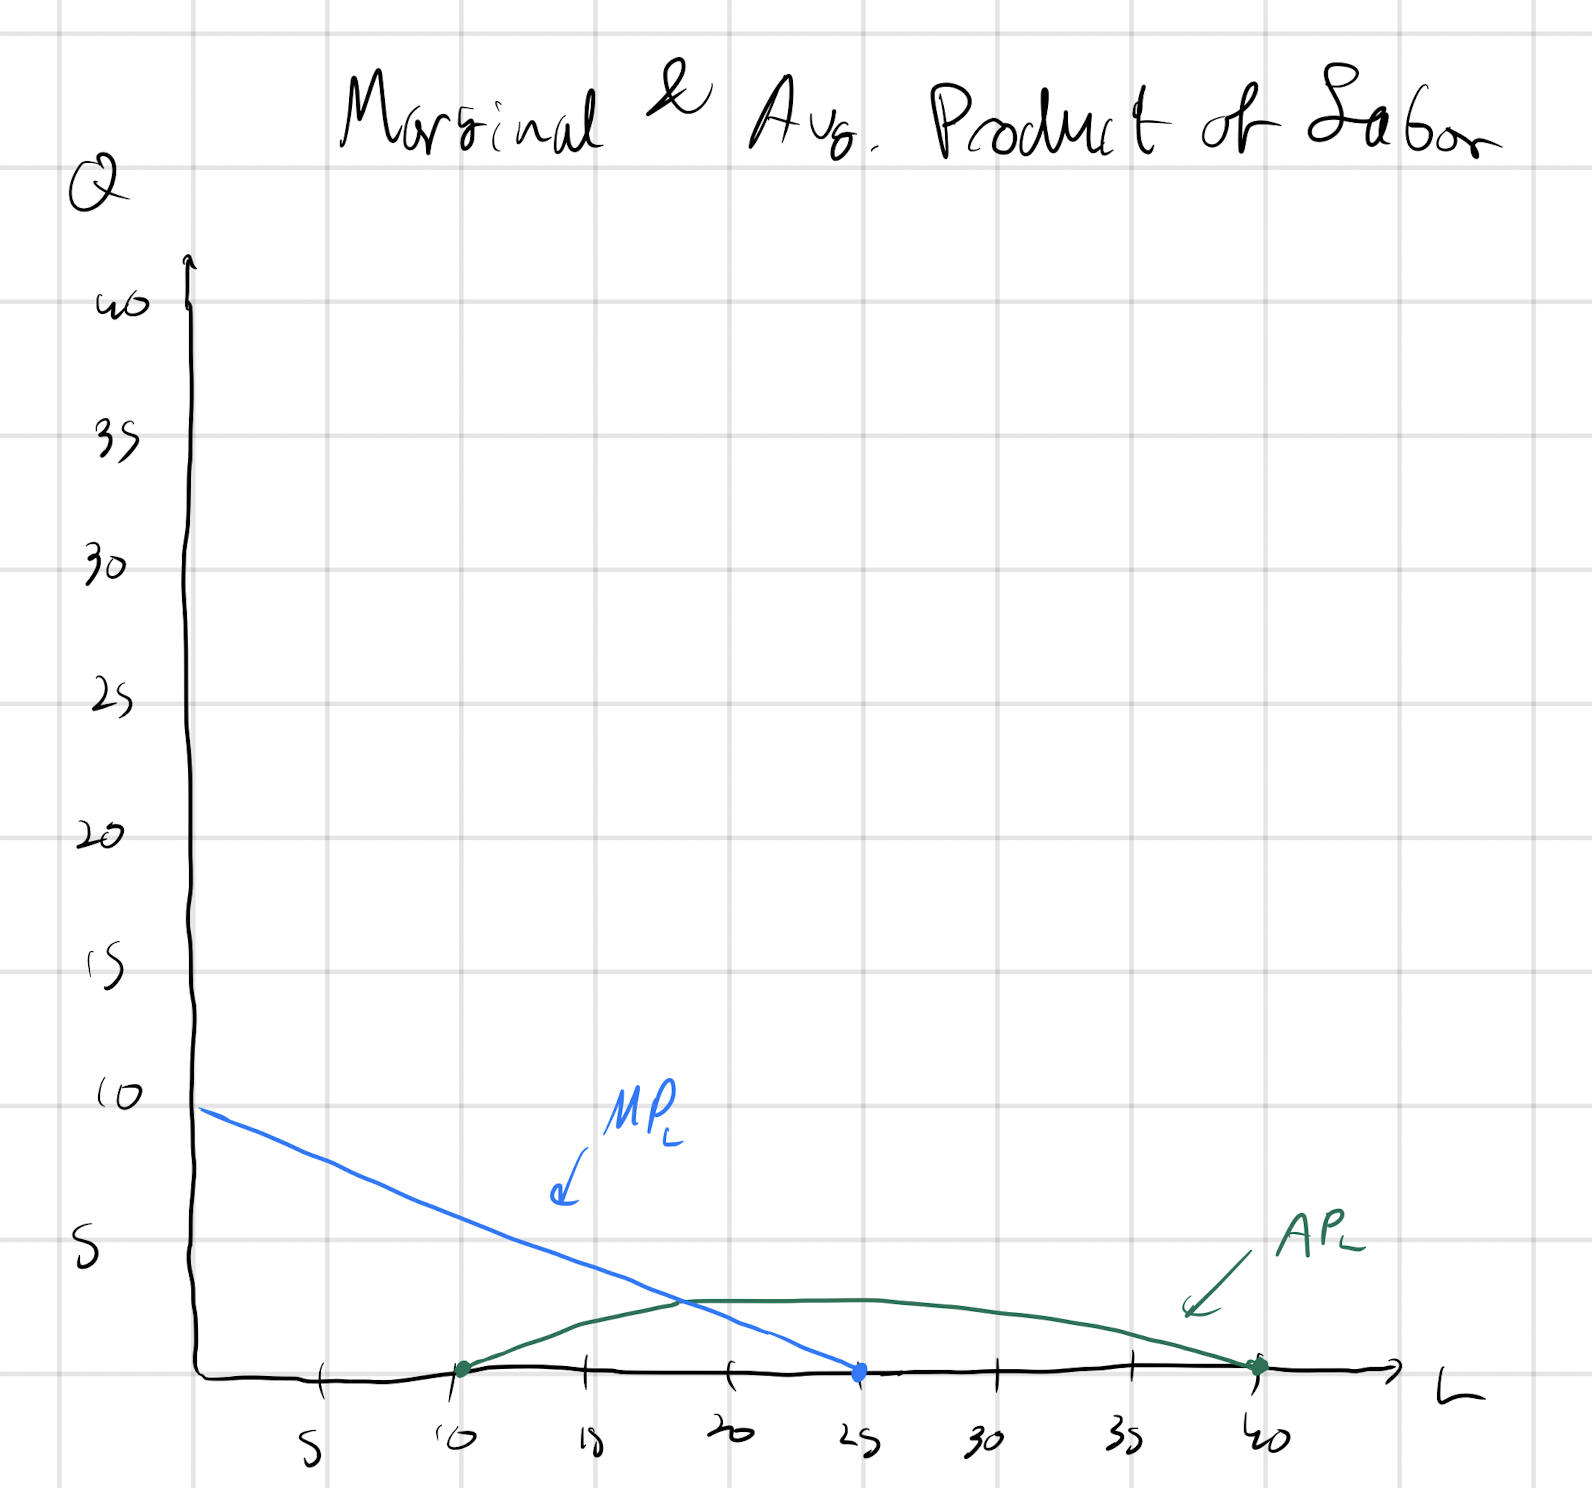
\includegraphics[width=10cm]{HW6Q1C}
\end{center}
At the level of labor where $MP_L = 0$, the business is at the maximal number of workers it can hire \textemdash afterwards, adding workers is detrimental to the firm's output.
\section{Marginal Product and Diminishing Returns}
\subsection*{Part A}
\begin{align*}
	MP_{K} &= \frac{\partial Q}{\partial K} \\
	&= A\alpha K^{\alpha - 1}L^{\beta} \\
	MP_L &= \frac{\partial Q}{\partial L} \\
	&= A\beta K^{\alpha}L^{\beta - 1}
\end{align*}
\subsection*{Part B}
\begin{align*}
	MRTS_{KL} &= \frac{MP_K}{MP_L} \\
	&= \frac{A\alpha K^{\alpha - 1}L^{\beta}}{A\beta K^{\alpha}L^{\beta - 1}} \\
	&= \frac{\alpha L}{\beta K} \\
	&= \frac{(1/3)(5)}{(2/3)(2)} \\
	&= \frac{5}{4}
\end{align*}
\section{Production Functions, Graphically}
\subsection*{Part A}
\begin{center}
	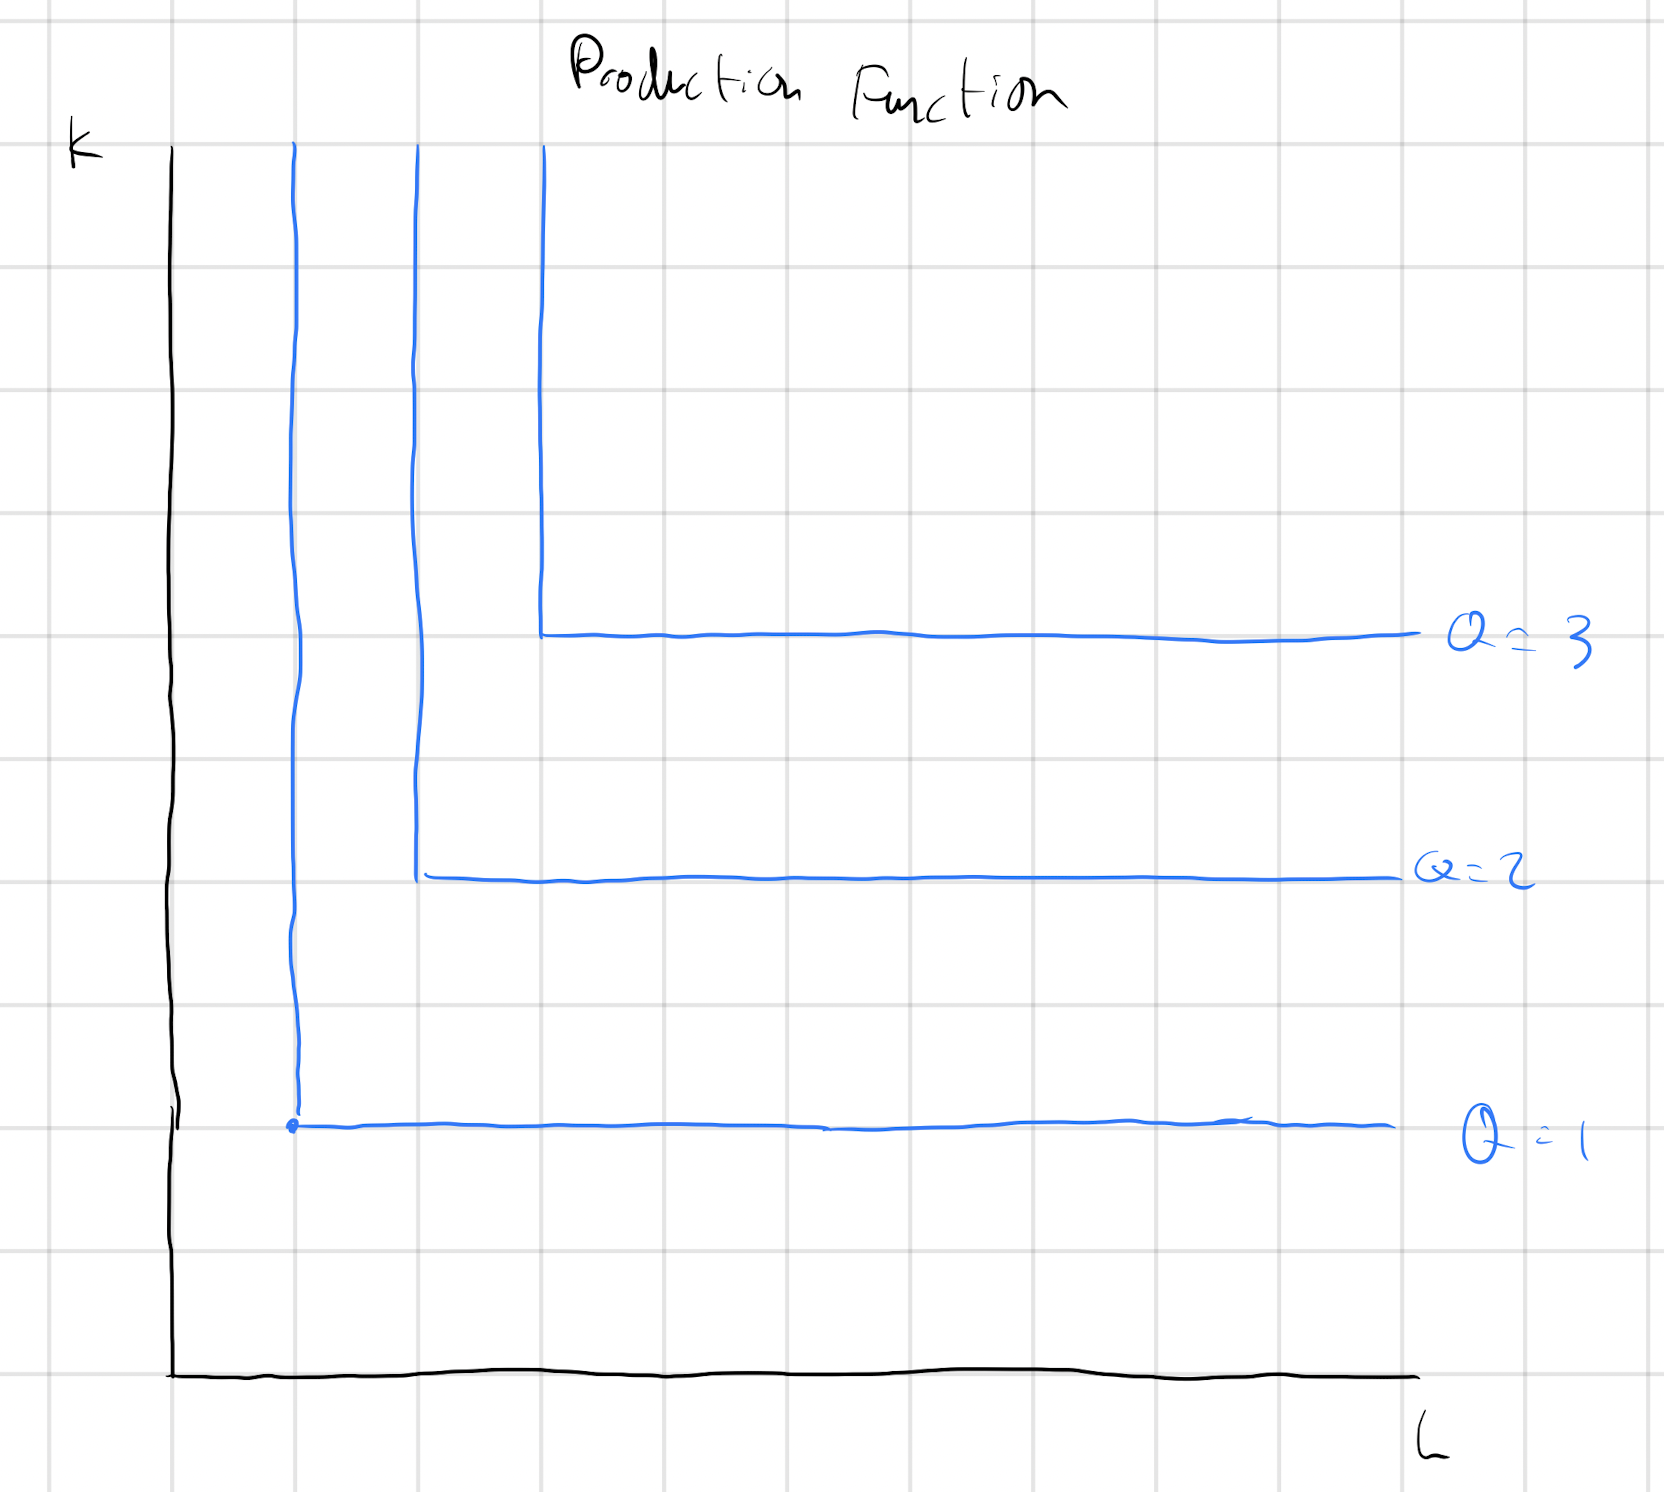
\includegraphics[width=10cm]{HW6Q3A}
\end{center}
\subsection*{Part B}
\begin{center}
	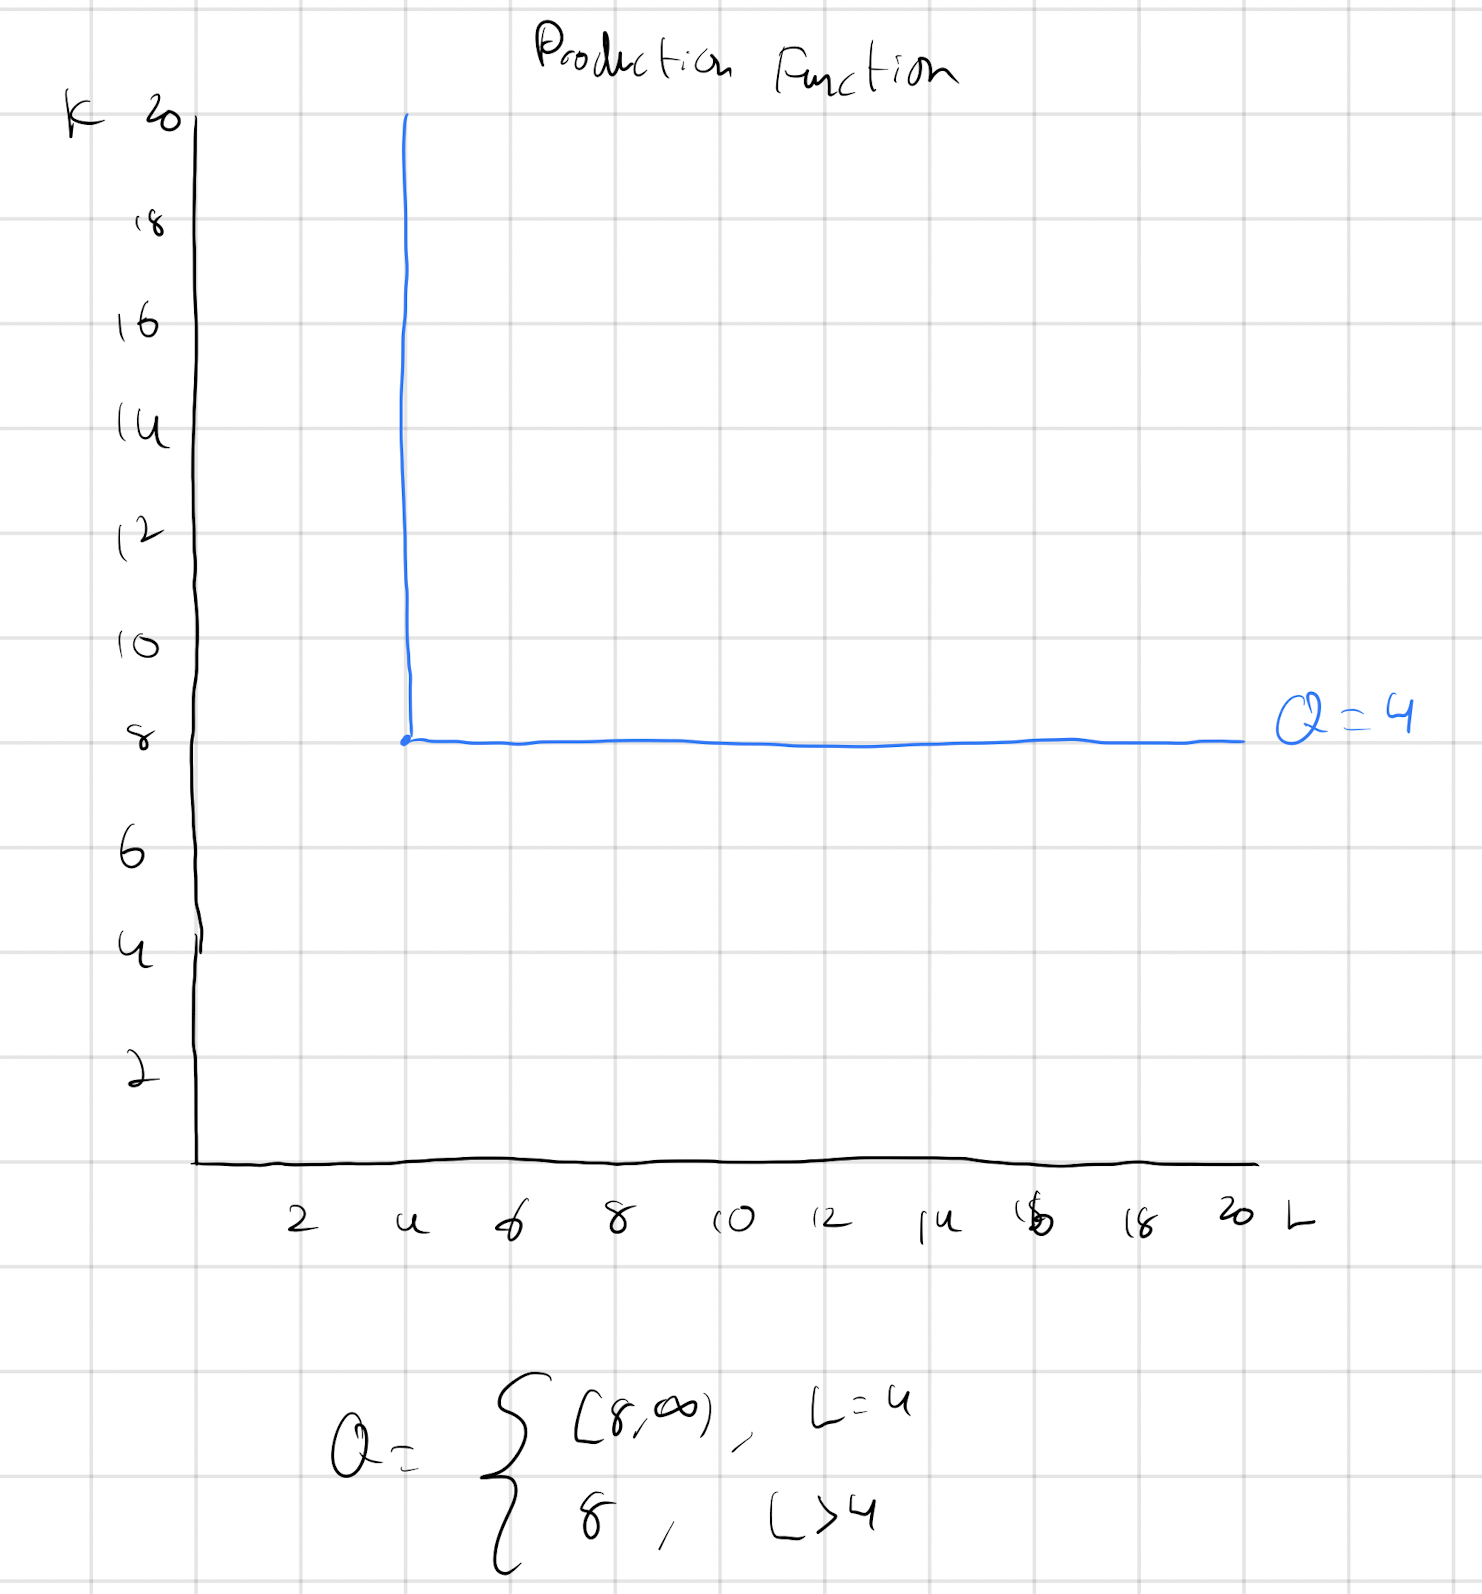
\includegraphics[width=10cm]{HW6Q3B}
\end{center}
\subsection*{Part C}
\begin{center}
	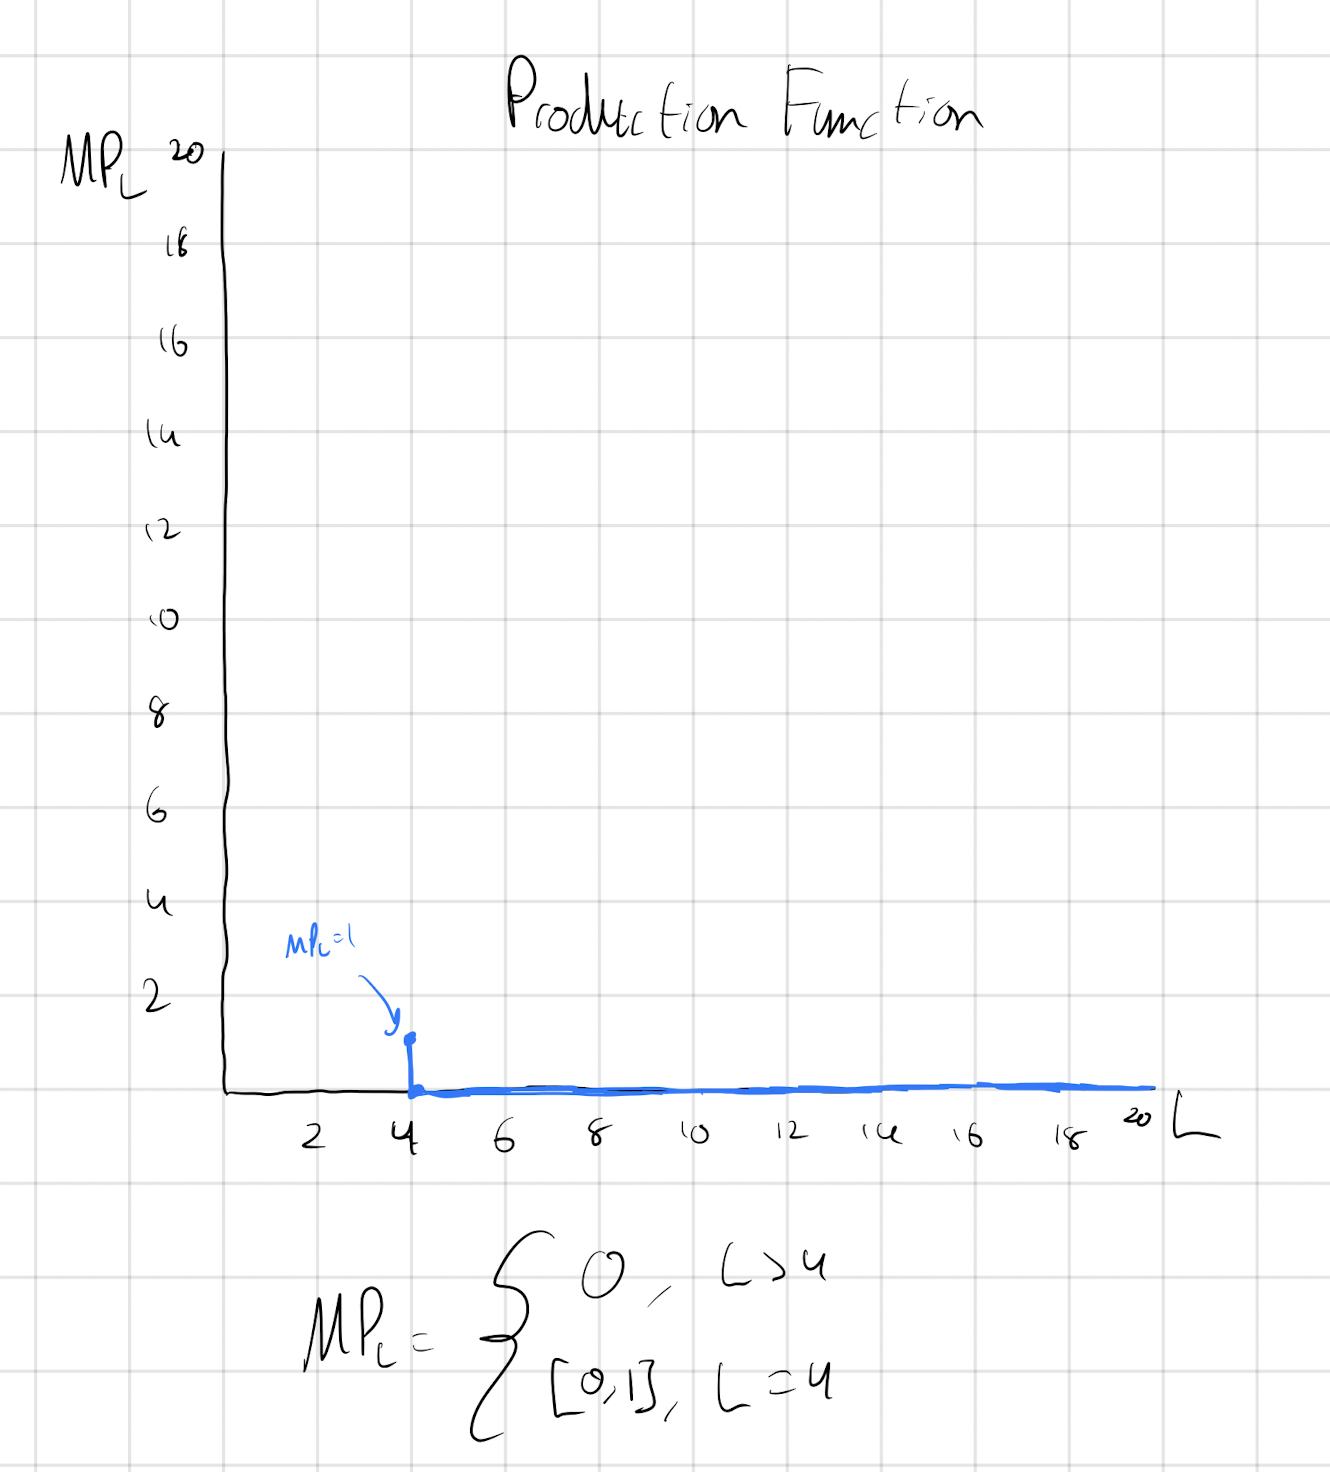
\includegraphics[width=10cm]{HW6Q3C}
\end{center}
\subsection*{Part D}
\begin{center}
	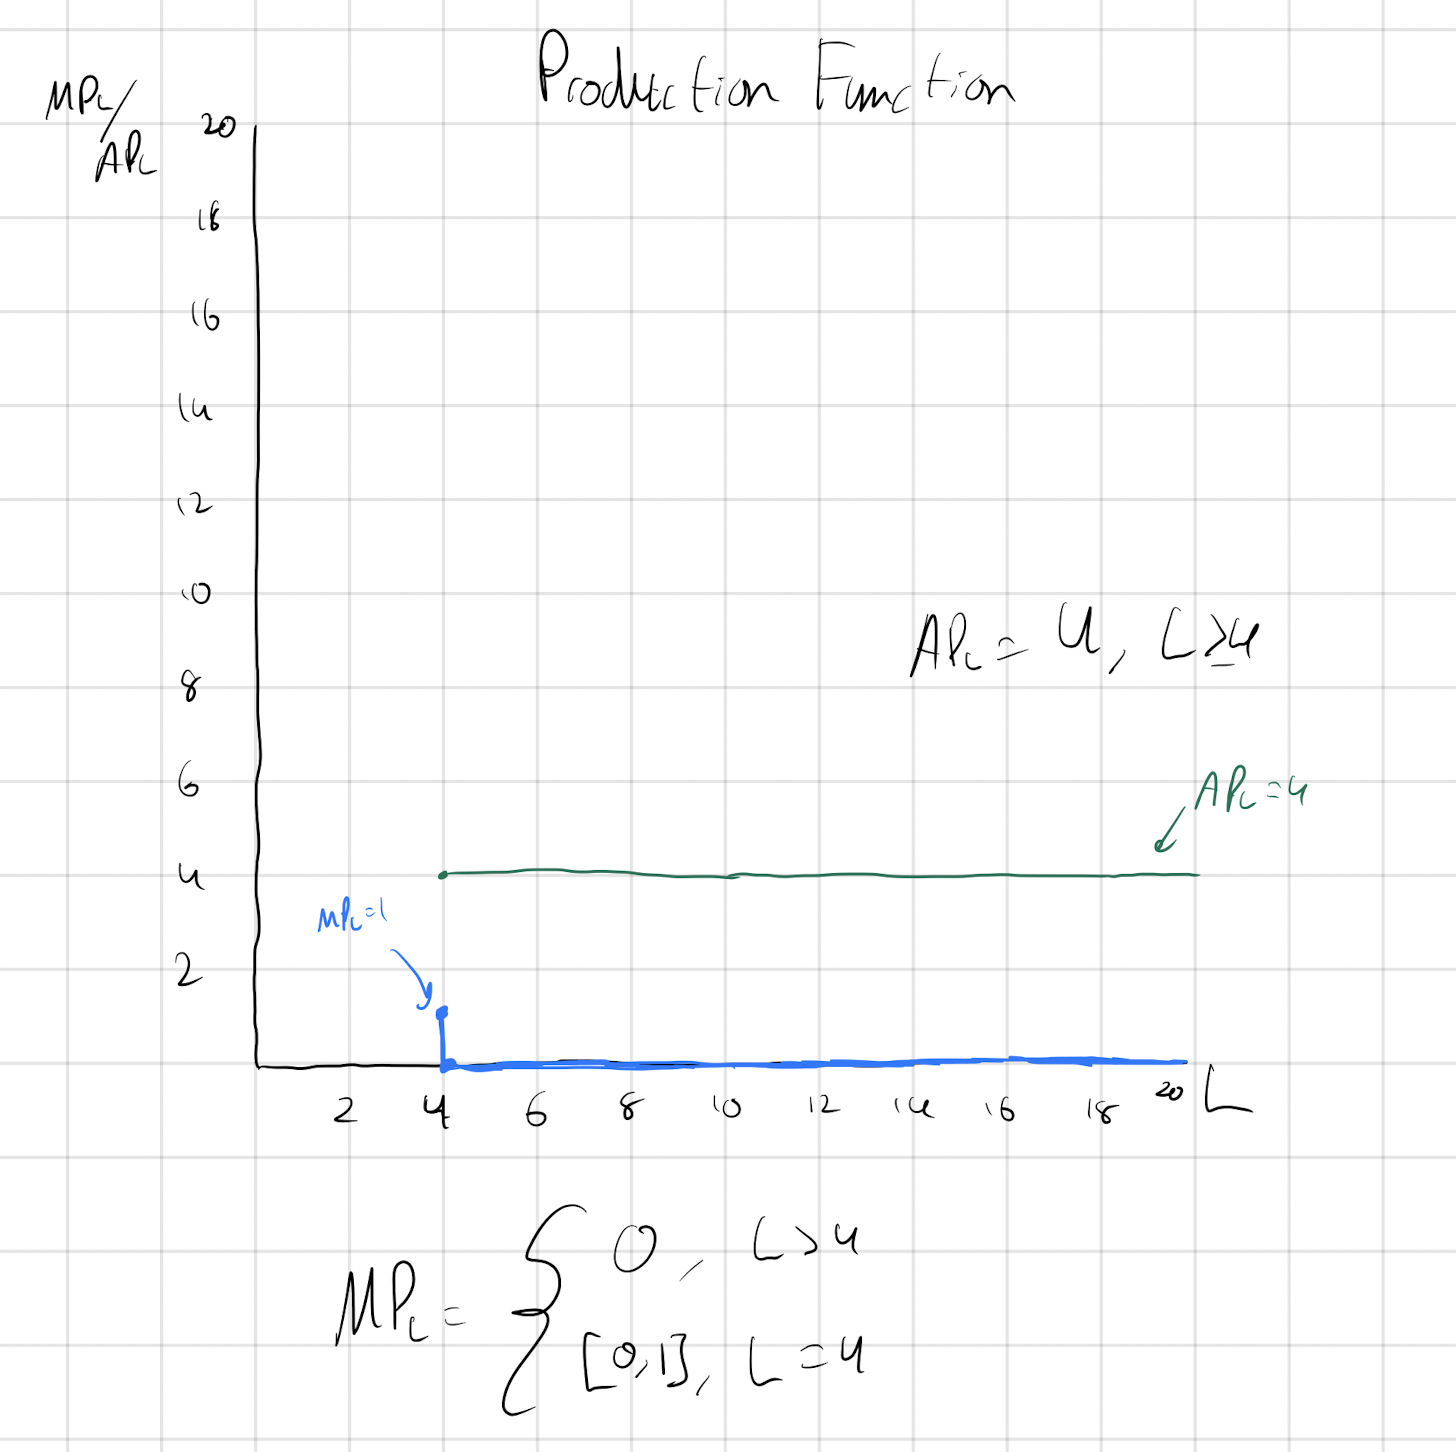
\includegraphics[width=10cm]{HW6Q3D}
\end{center}
\section{Isoquants, Graphically}
\begin{center}
	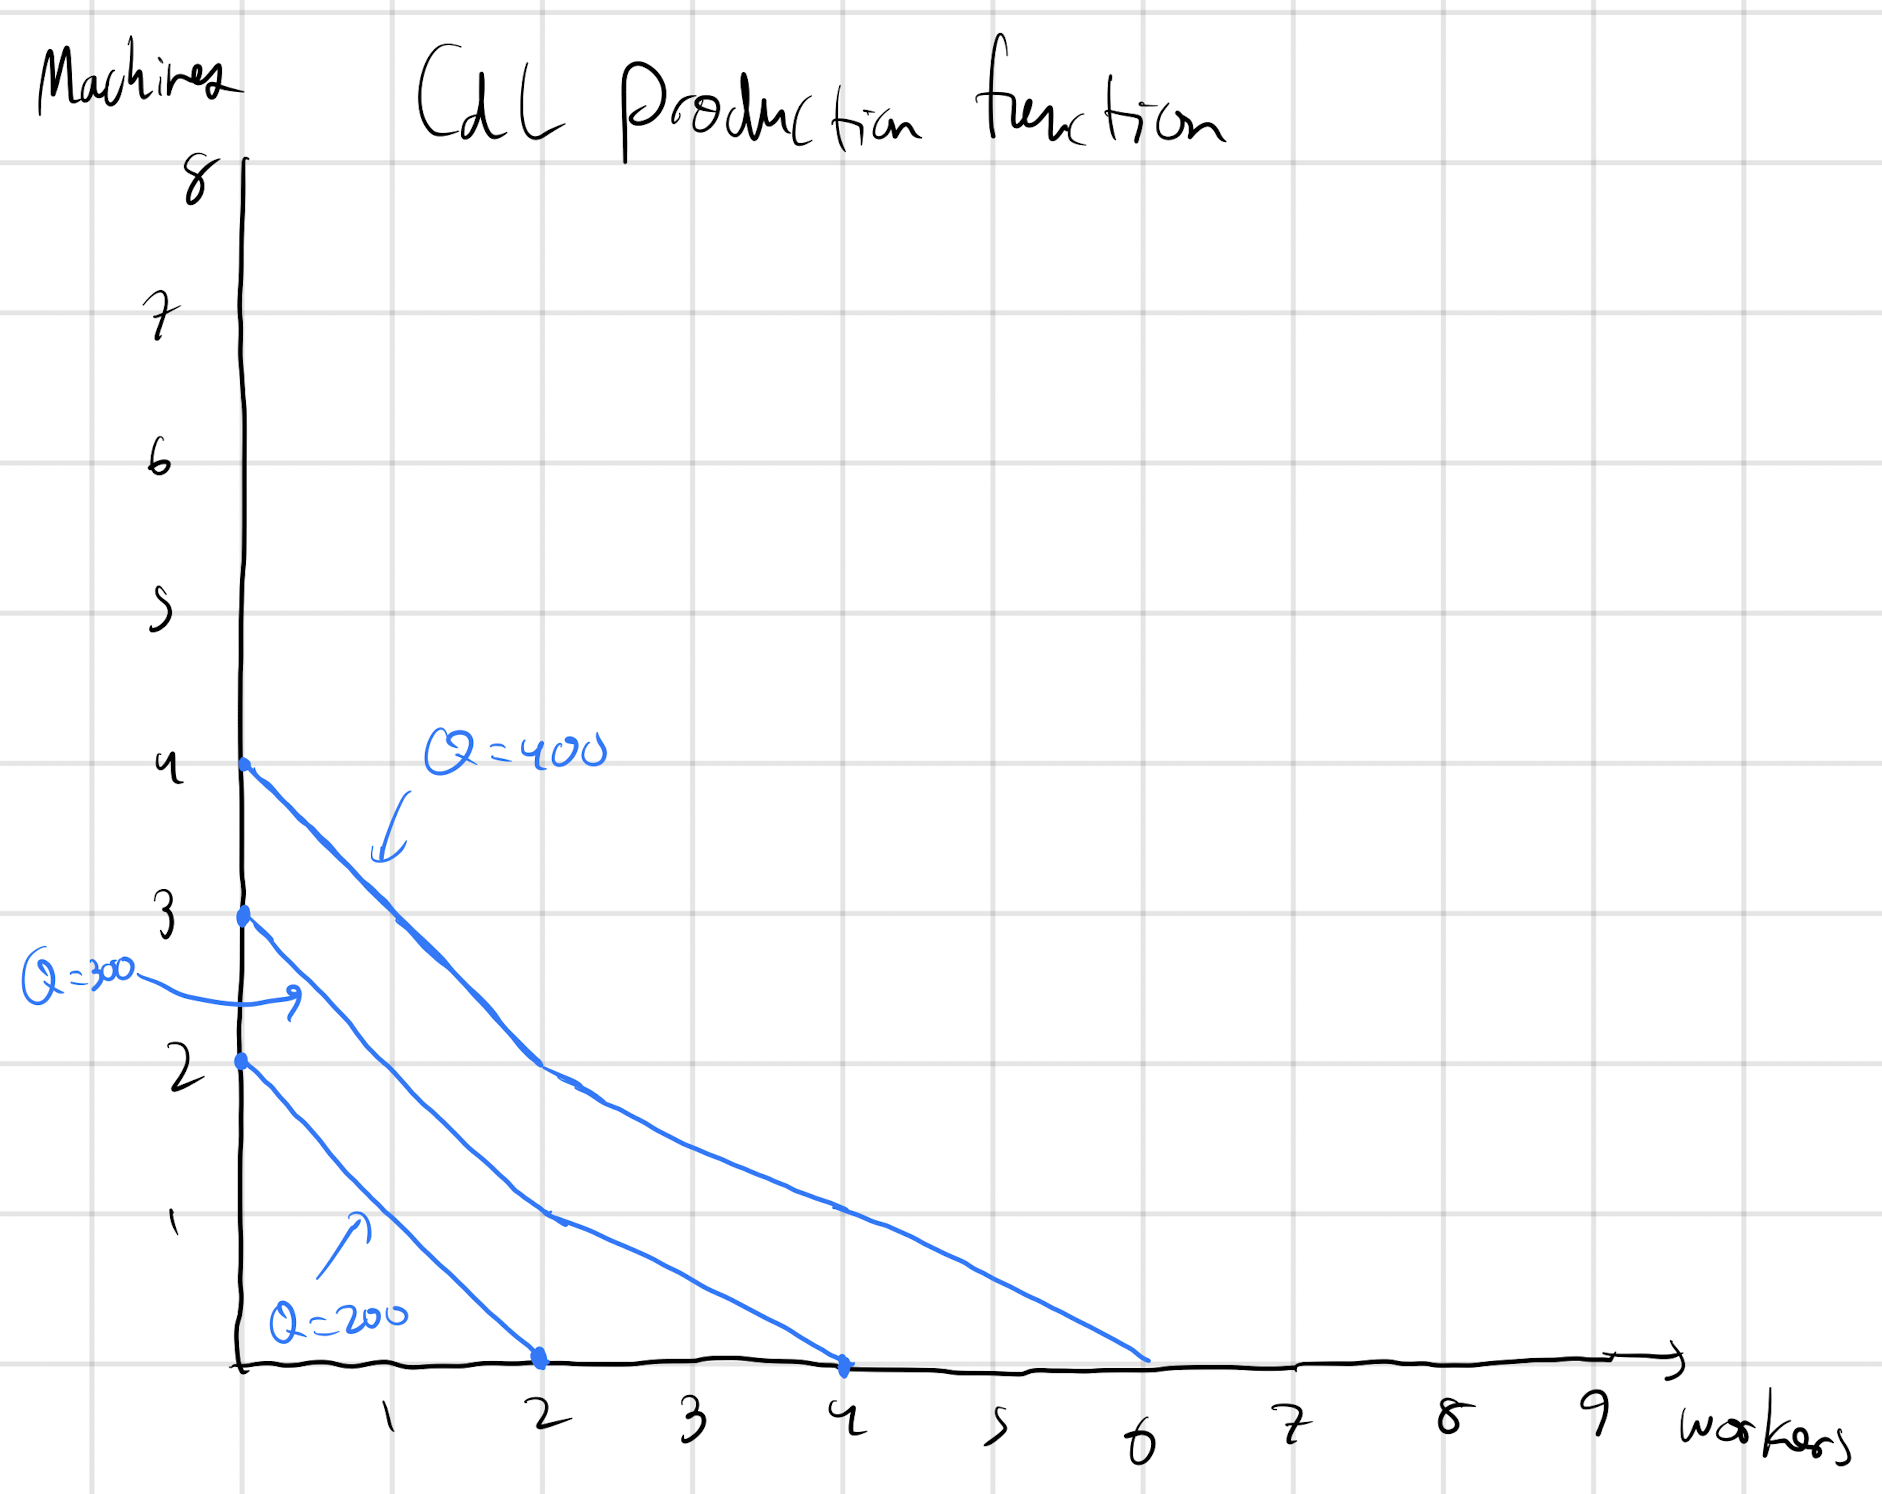
\includegraphics[width=10cm]{HW6Q4}
\end{center}
\section{Production Functions in Tables}
\subsection*{Part A}
The $MP_L$ of Hawg Wild's nephew will be $408-347 = 61$ new diners served.
\subsection*{Part B}
The production function does \textbf{not} violate the law of diminishing marginal product because the marginal product of \textit{capital} is lower between when $K=1$ and $K=5$, as well as the fact that the $MP_L$ of the fifth laborer is lower than the $MP_L$ of the first labor at both points.
\subsection*{Part C}
The $MP_K$ is equal to $387-347 = 40$ new diners served.
\subsection*{Part D}
\begin{align*}
	\frac{MP_K}{R} &= \frac{40}{8} \\
	\frac{MP_L}{W} &= \frac{61}{12} \\
	\frac{MP_L}{W} &> \frac{MP_K}{R}
\end{align*}
Therefore, Billy should \textbf{hire an additional worker}.
\section{Cost Minimization, Graph}
\subsection*{Part A}
Yes, the firm can produce 248K units of output at \$336, by using the cost curve that is farthest from the origin on the original graph.
\subsection*{Part B}
The minimum cost for which 248K units can be produced is $(10)(24) = \$240 $
\subsection*{Part C}
\begin{align*}
	\frac{MP_K}{MP_L} &= \frac{R}{L} \\
	MP_K &= MP_L \frac{R}{L} \\
	&= (400)\frac{24}{36} \\
	&= \boxed{266.67}
\end{align*}
\section{Cost Minimization, Moving Decisions}
\subsection*{Part A}
\begin{center}
	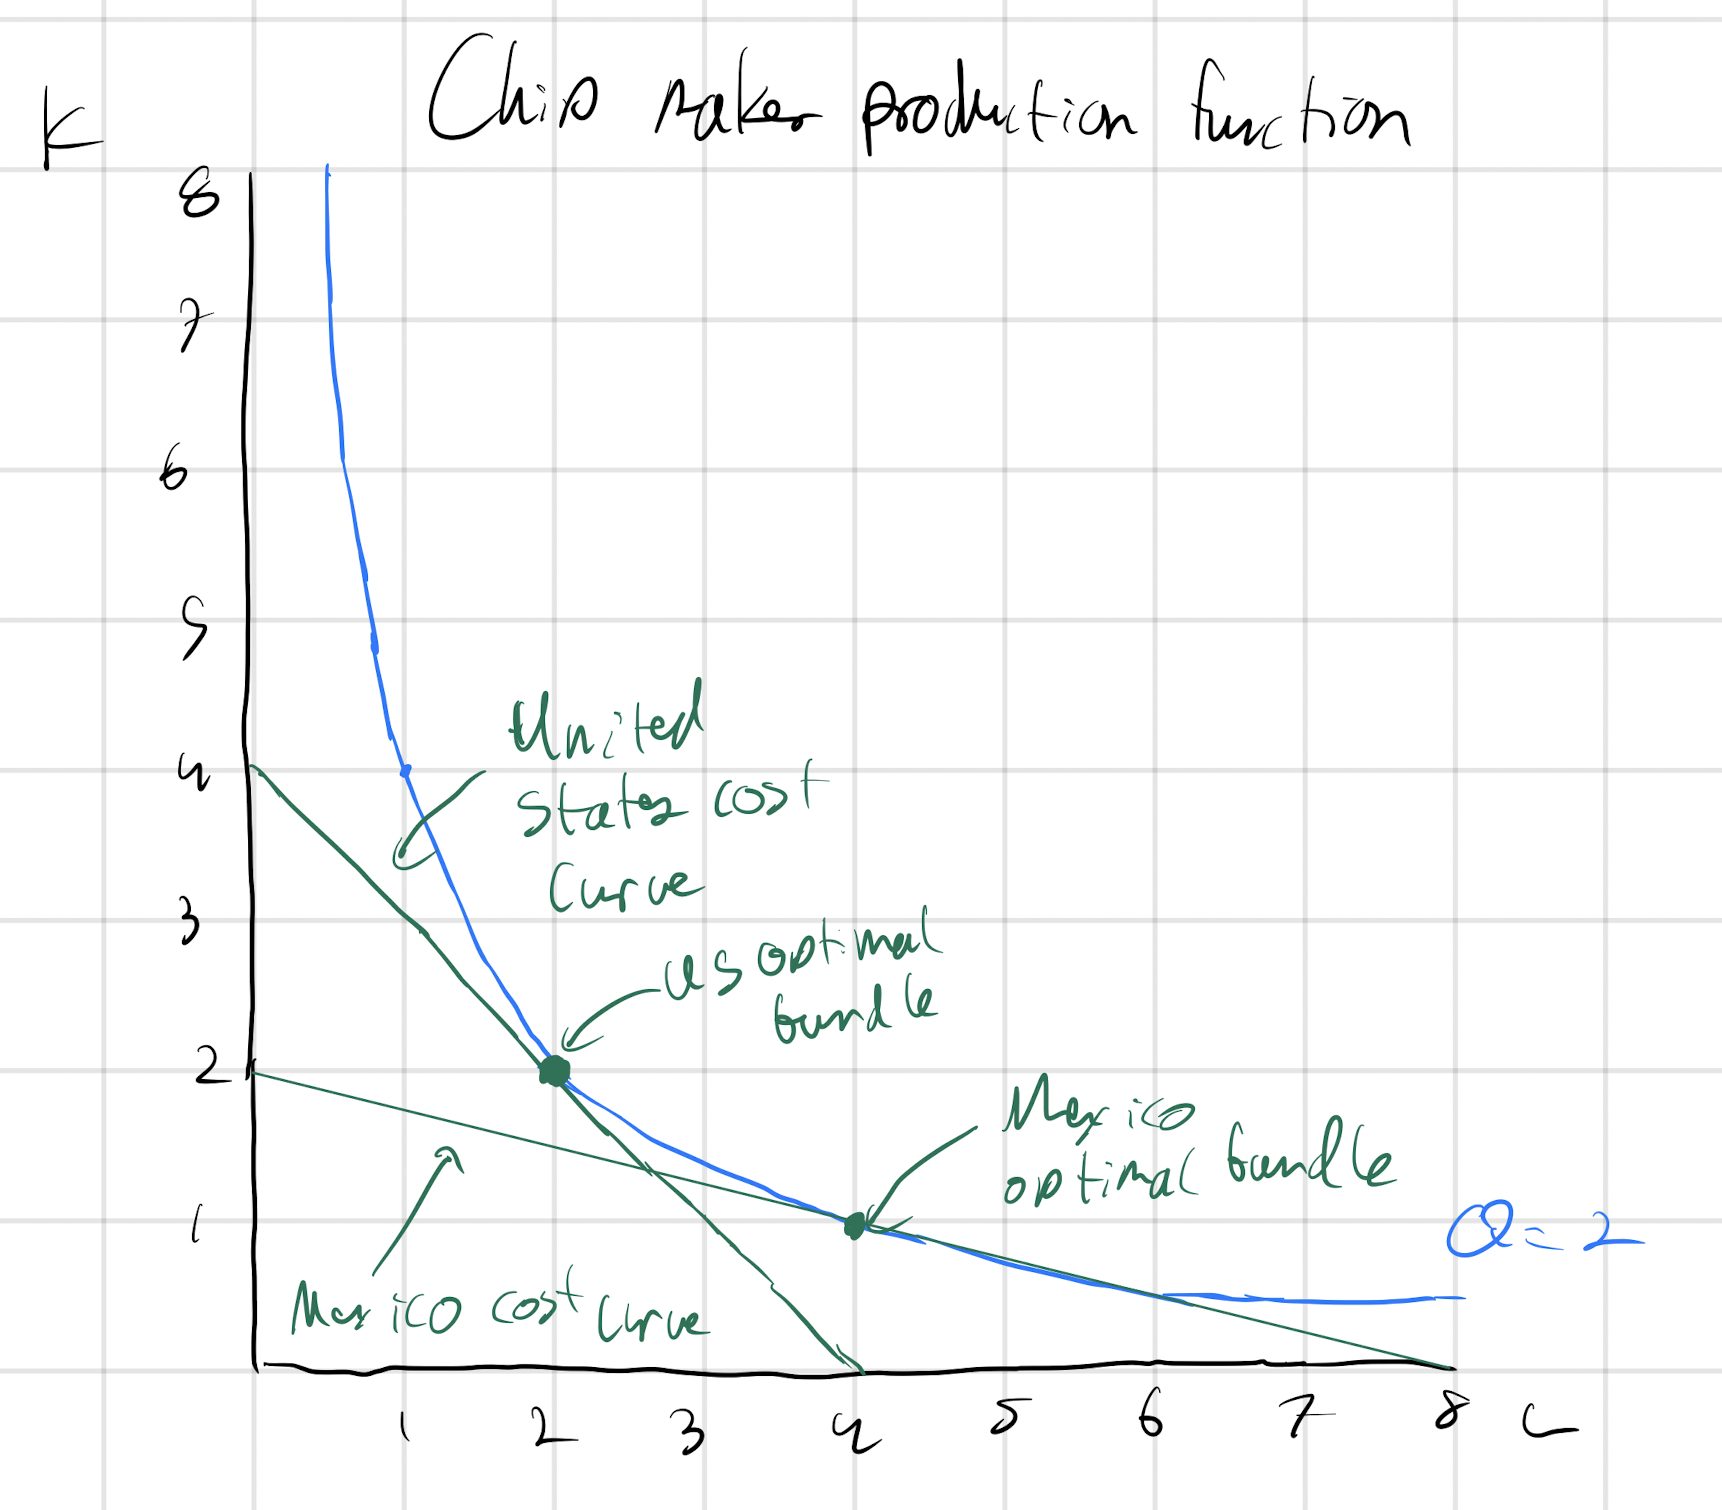
\includegraphics[width=10cm]{HW6Q7A}
\end{center}
\subsection*{Part B}
It is apparent here that the optimal decision for the firm is to move to Mexico, where the cost of capital might be the same but the wage is lower, so the cost curve is closer to the origin.
\subsection*{Part C}
\begin{align*}
	\frac{MP_K}{MP_L} &= \frac{R_1}{W_1} \\
	\frac{MP_K}{MP_L} &= \frac{R_2}{W_2} \\
	\frac{L}{K} &= \frac{10}{10} \\
	\frac{L}{K} &= \frac{10}{2.5} \\
	100 &= (L)^{0.5}(L)^{0.5} \\
	L_1 &= 100 \\
	K_1 &= 100 \\
	C_1 &= (10)(L_1) + (10)(K_1) \\
	&= \boxed{\$2000} \\
	100 &= (K)^{0.5}(4K)^{0.5} \\
	100 &= 2K \\
	K_2 &= 50 \\
	L_2 &= 200 \\
	C_2 &= (2.5)(L_2) + (10)(K_2) \\
	&= \boxed{\$1000} 
\end{align*}
\section{Cost Minimization, Computations}
\begin{align*}
	Q &= K + 4\sqrt{L} \\
	C &= 20K + 10L \\
	\frac{MP_K}{MP_L} &= \frac{R}{L} \\
	\frac{\sqrt{L}}{2} &= 2 \\
	100 &= K + (4)(4) \\
	K &= 84 \\
	L &= 16
\end{align*}
\section{Cost Minimization, Graphs}
\begin{center}
	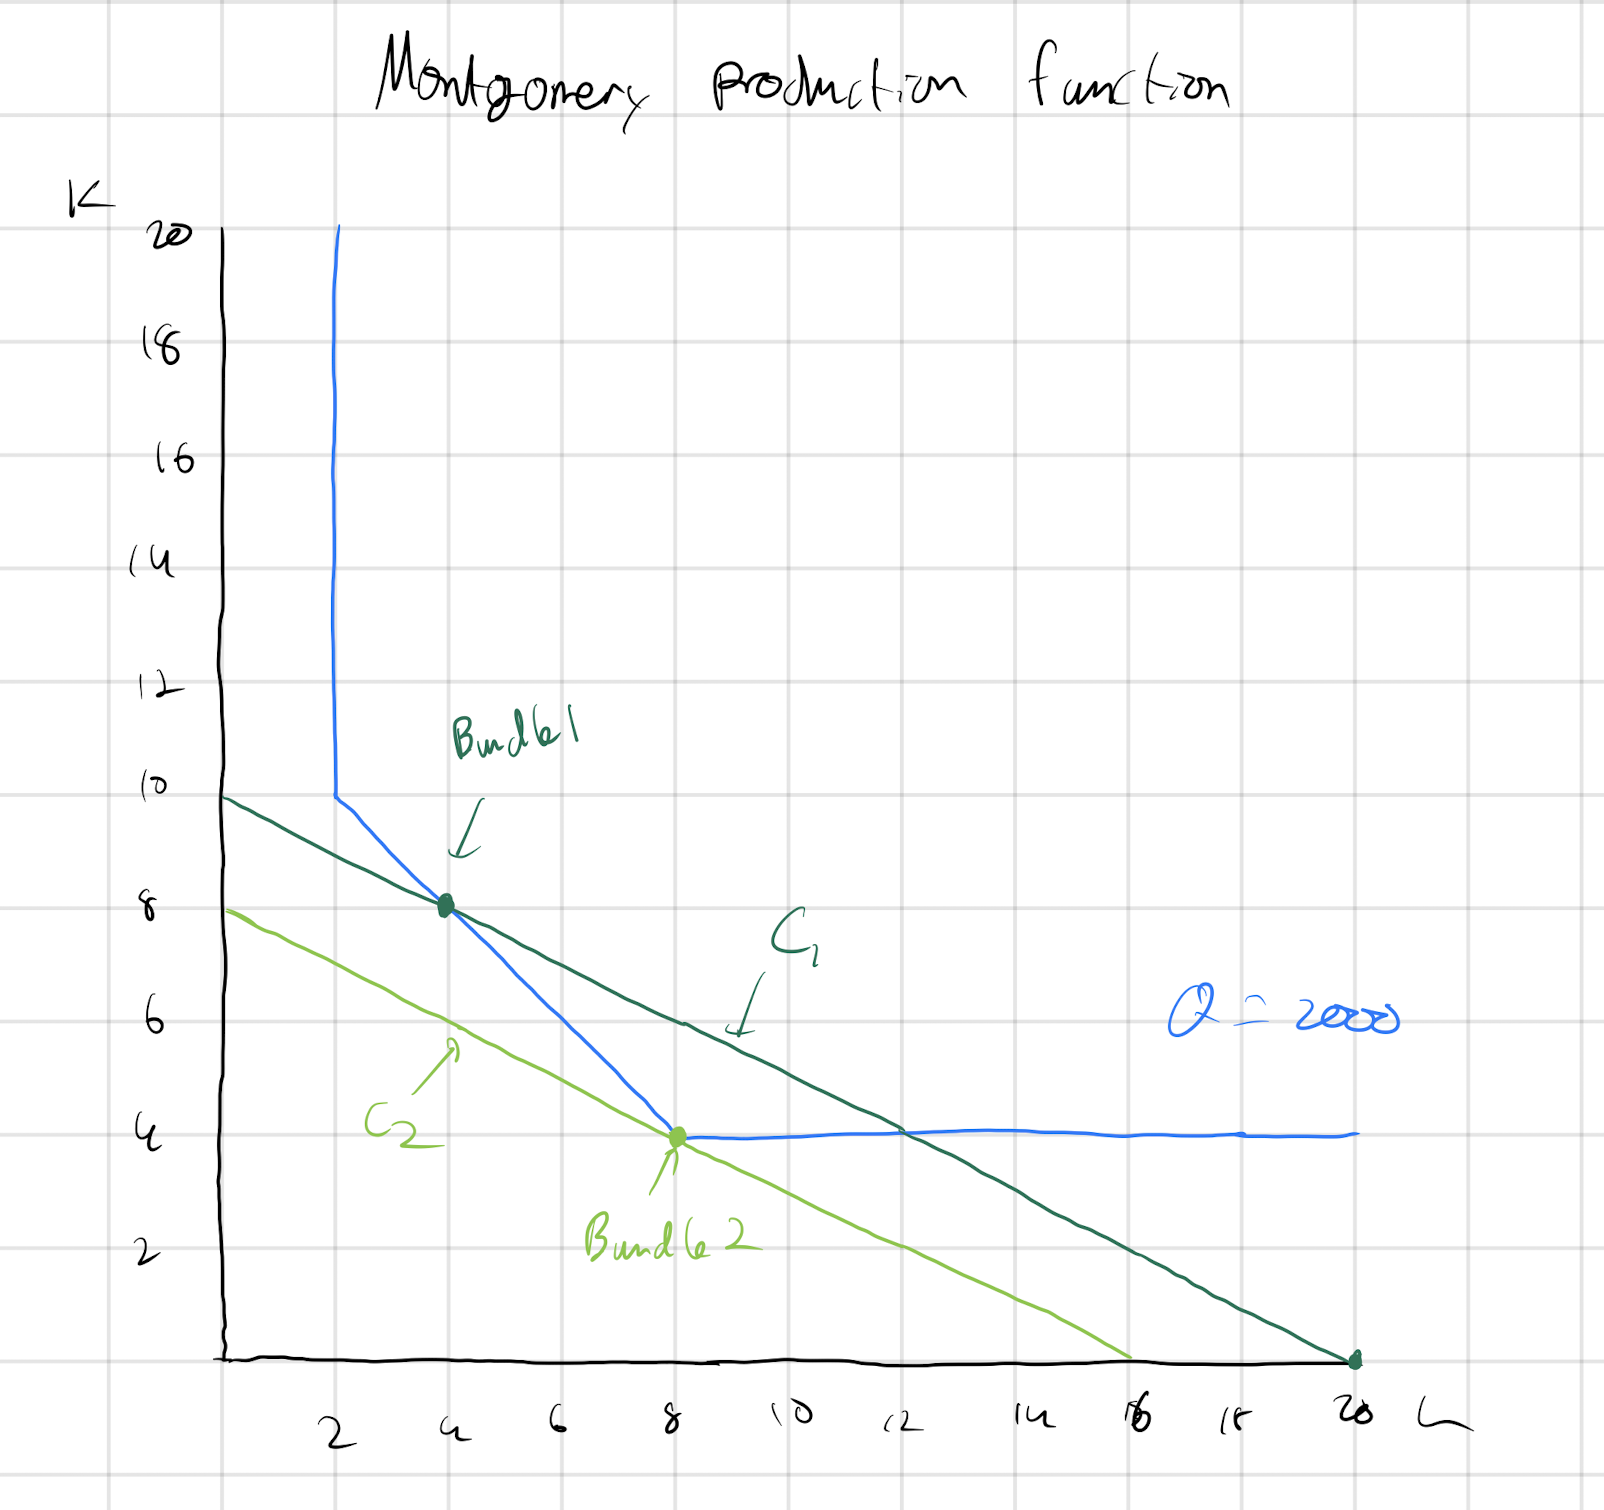
\includegraphics[width=10cm]{HW6Q9}
\end{center}
As seen in the graph above, Montgomery can reduce his costs and still produce the desired output by using 8 workers and 4 units of capital, with a total cost of $(16)(20) = \$320$ rather than the \$400 that he is currently using.
\pagebreak
\section{Corner Solutions}
\begin{align*}
	\frac{MP_K}{MP_L} &= \frac{R}{W} \\
	\frac{1}{\sqrt{K}} &= \frac{1}{W} \\
	\sqrt{K} &= W \\
	10 &= 2W + L
\end{align*}
Yes, it is possible for the wage rate to be high enough where it is optimal to use capital — namely, if the wage rate is greater than or equal to 5, then it is optimal to entirely use capital. The reason for this is that the marginal product of labor is constant, meaning that it is possible for the wage rate to be higher than the value of the marginal product of capital, meaning it is infeasible to hire any workers.
\begin{center}
	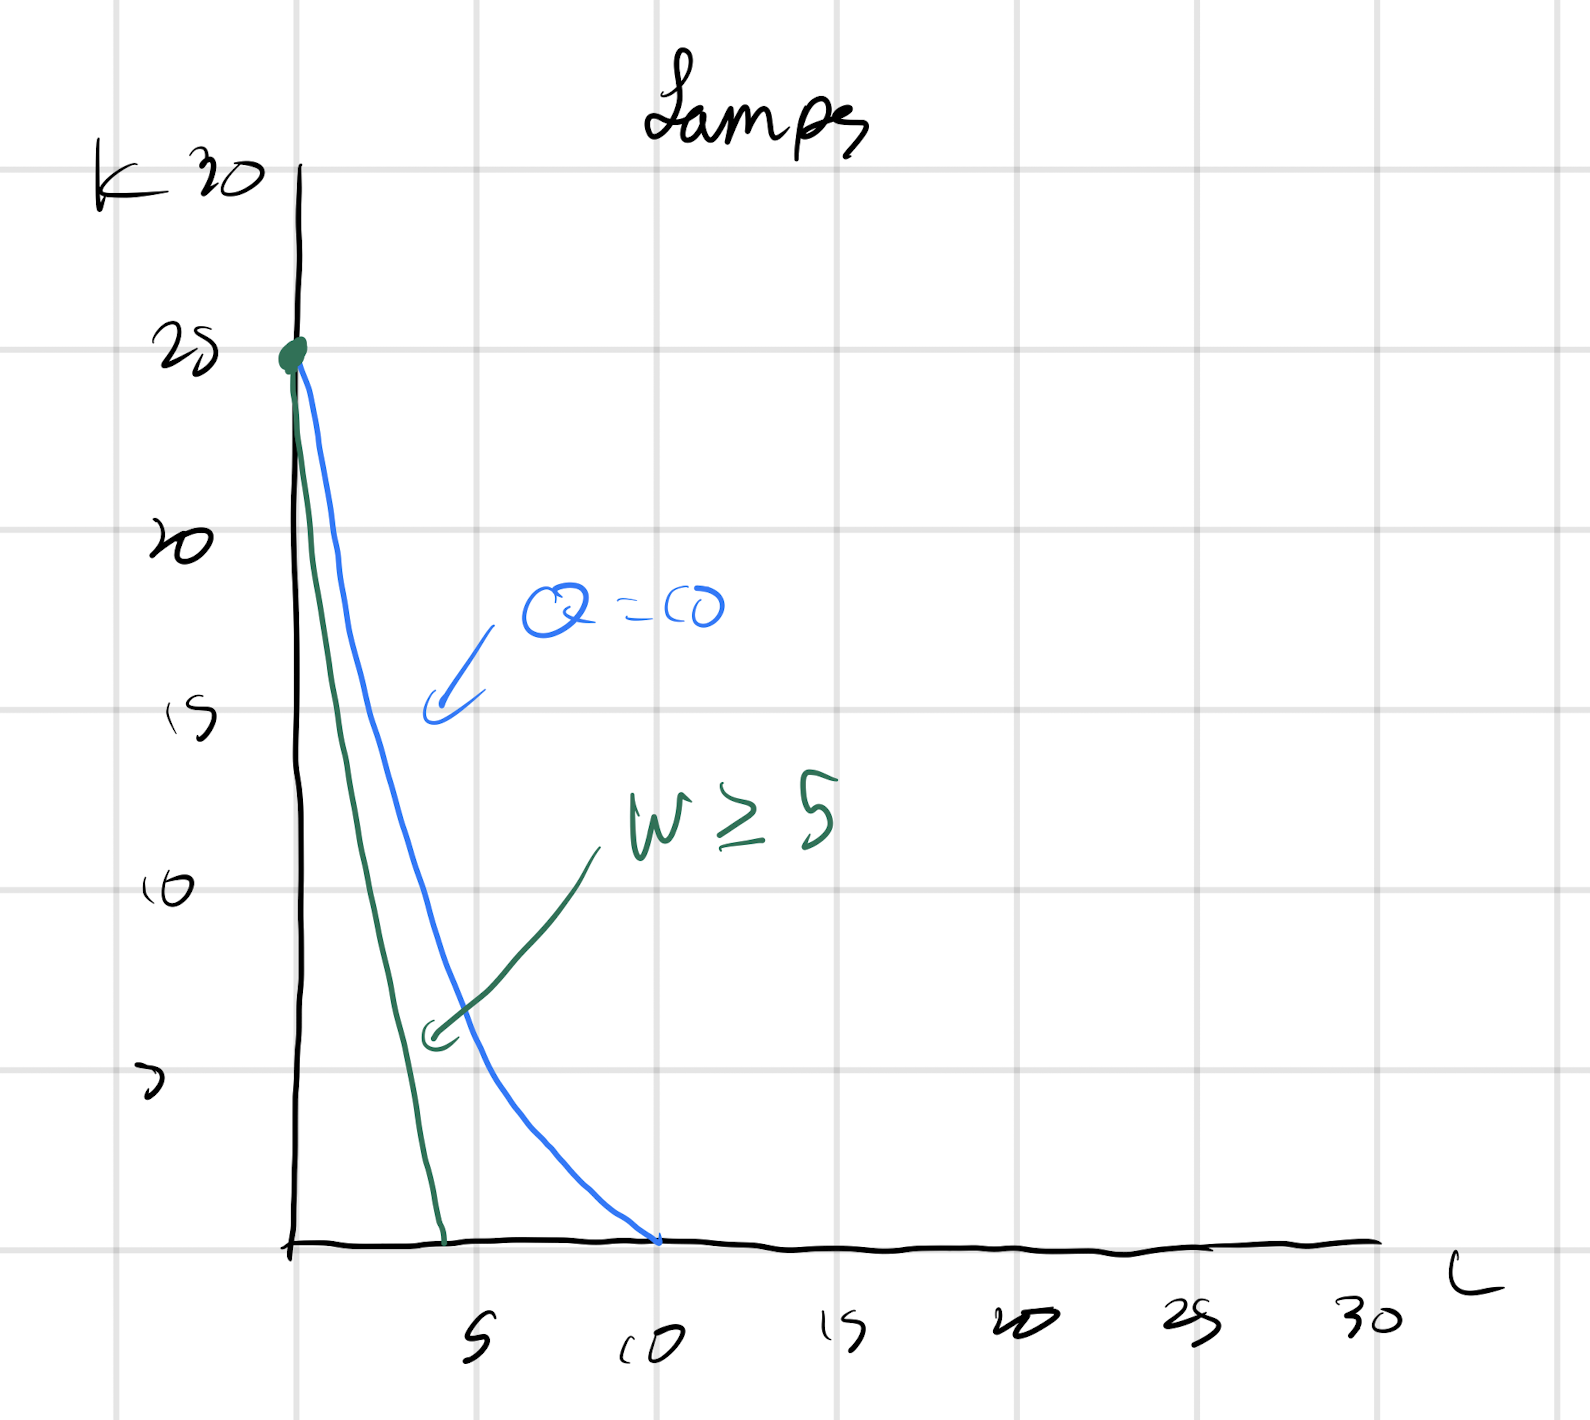
\includegraphics[width=10cm]{HW6Q10}
\end{center}
\pagebreak
\section{Conceptual Questions}
\begin{itemize}
	\item True \textemdash if the marginal product of labor is increasing, then the average product of labor will be ``weighed down'' by the marginal products of earlier workers, meaning that the $AP_L$ curve will be below the $MP_L$ curve.
	\item False \textemdash since the wage rate per worker relative to a unit of capital is lower than the productivity per worker relative to capital, it is efficient to hire more workers because they are more productive relative to capital than the price the company pays, rather than lay off workers to hire more capital.
	\item True \textemdash if the marginal rate of technical substitution is even more biased in favor of capital, then it is possible for the firm to use entirely capital. See the picture below.
\end{itemize}
\begin{center}
	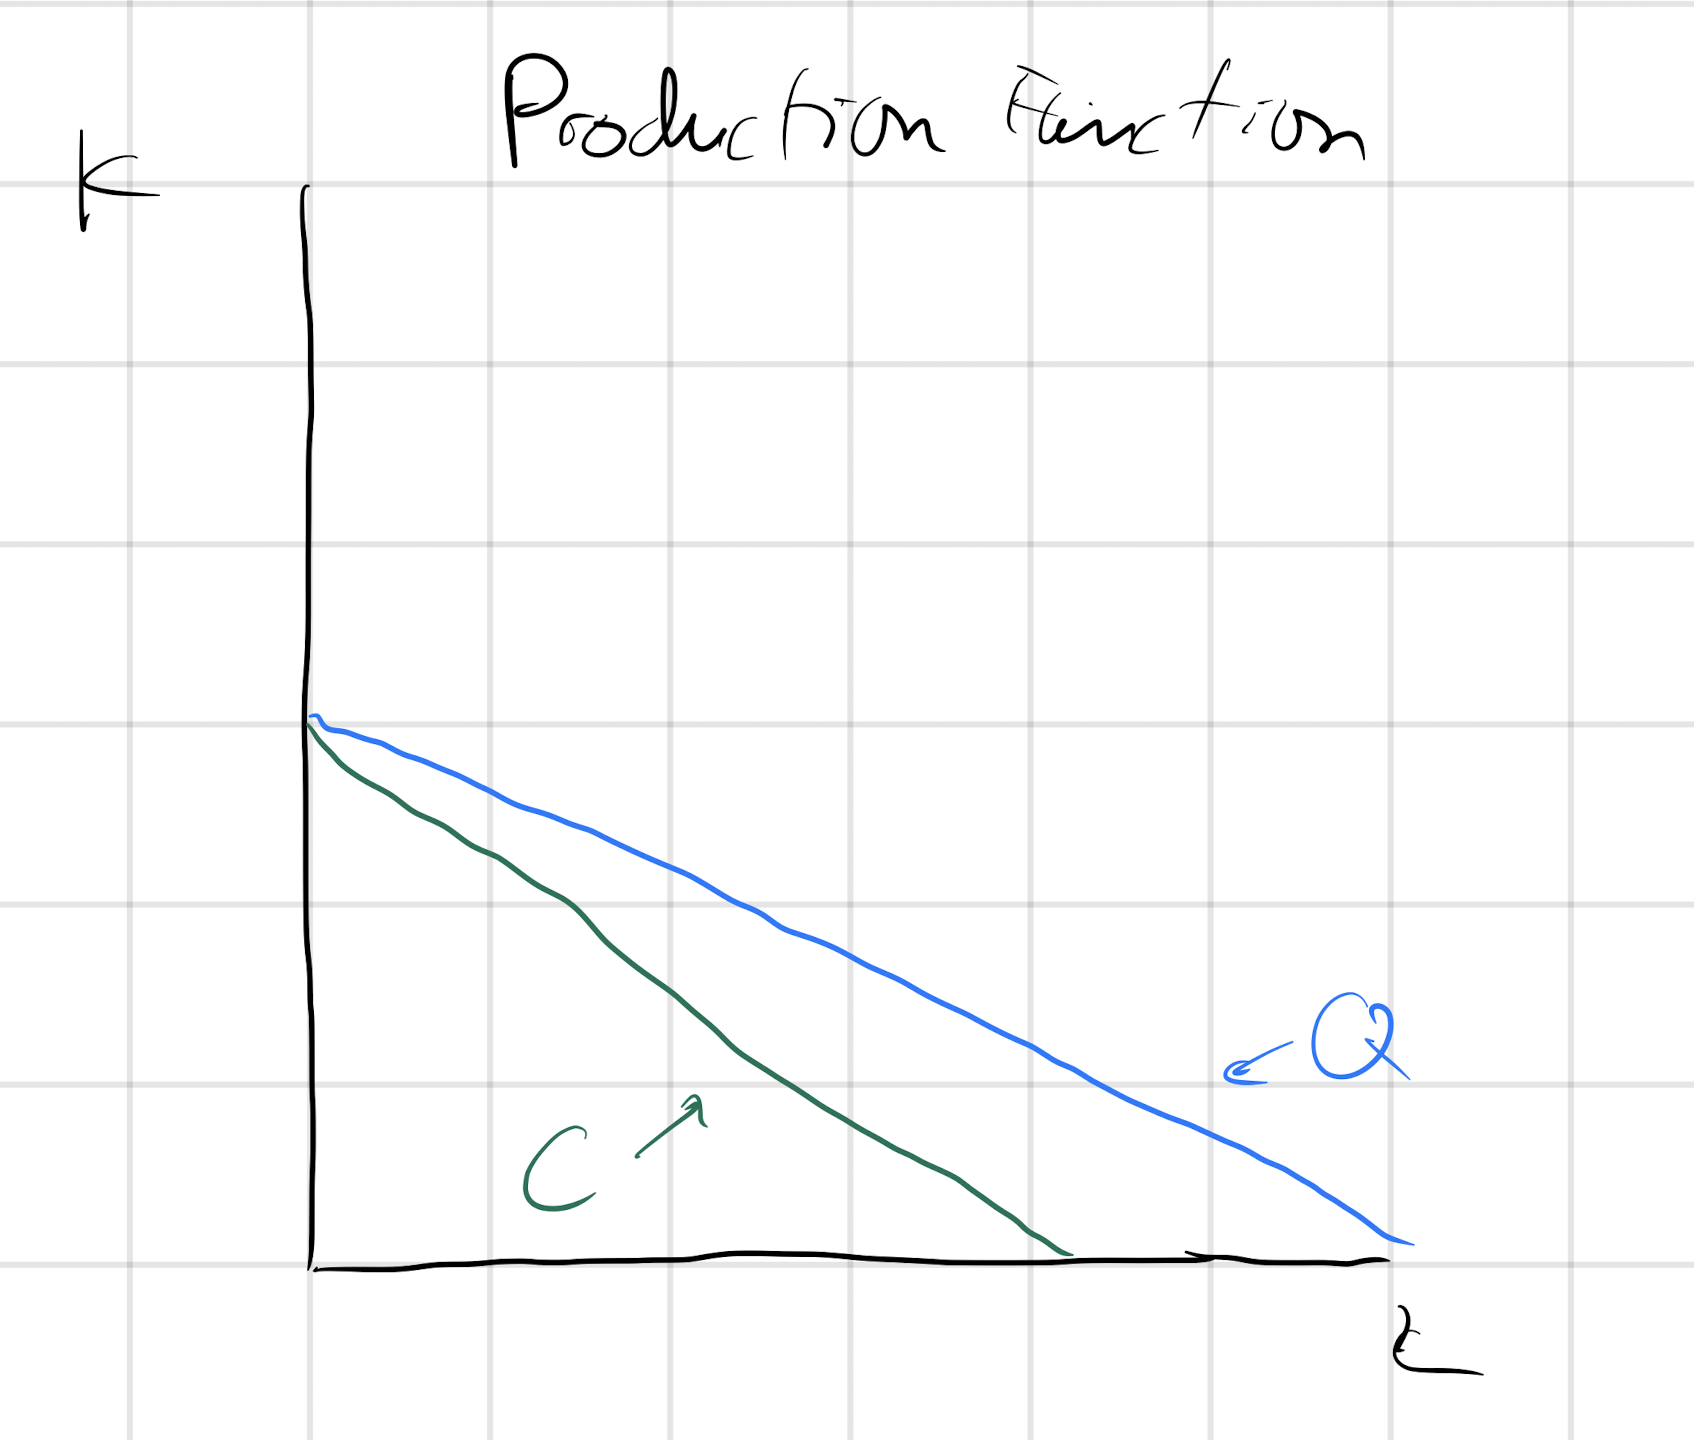
\includegraphics[width=10cm]{HW6Q11C}
\end{center}
\end{document}